%%% -*- mode:latex; -*-
\documentclass[a4paper]{report}

\usepackage[utf8x]{inputenc}
\usepackage[greek,french,english,macedonian]{babel}



\usepackage{amsmath}
\usepackage{amsfonts}%
\usepackage{graphicx}
\usepackage{multirow}
\usepackage{epsfig}
\usepackage{url}
\usepackage{amsthm}

\usepackage{graphicx}
\usepackage{float}
\usepackage[lined,linesnumbered,ruled,vlined]{algorithm2e}
\usepackage{epsfig}
\usepackage{subfig}
\usepackage{color}


\newtheorem{theorem}{\cyr \CYRT\cyre\cyro\cyrr\cyre\cyrm\cyra}
\newtheorem{corollary}[theorem]{\cyr \CYRP\cyro\cyrs\cyrl\cyre\cyrd\cyri\cyrc\cyra}
\newtheorem{lemma}[theorem]{\cyr \CYRL\cyre\cyrm\cyra}



\usepackage{imakeidx}
\makeindex

\title{\selectlanguage{macedonian}Пример за употреба}
\author{Стојан Трајановски\\\texttt{stojan.trajanovski@gmail.com}}
\begin{document}
\maketitle

\begin{abstract}
А, Б, В, Г, Д
\end{abstract}

\selectlanguage{macedonian}

\tableofcontents


\chapter{Вовед}

\section{Азбука}
Азбука големи букви:\\
 А, Б, В, Г, Д, Ѓ, Е, Ж, З, S, И,\\
  Ј, К, Л, Љ, М, Н, Њ, О, П, Р, С,\\Т, Ќ, У, Ф, Х, Ц, Ч, Џ, Ш\\
 
 Азбука мали букви:\\
 а, б, в, г, д, ѓ, е, ж, з, ѕ, и,\\ ј, к, л, љ, м, н, њ, о, п, р, с,\\ т, ќ, у, ф, х, ц, ч, џ, ш\\
 
 
 
 
\textit{Азбука во италик големи букви: \\
А, Б, В, Г, Д, Ѓ, Е, Ж, З, S, И,\\ Ј, К, Л, Љ, М, Н, Њ, О, П, Р, С,\\ Т, Ќ, У, Ф, Х, Ц, Ч, Џ, Ш}\\

\textit{Азбука во италик мали букви:\\
 а, б, в, г, д, ѓ, е, ж, з, ѕ, и,\\ ј, к, c, љ, м, н, њ, о, п, р, с,\\ т, ќ, у, ф, х, ц, ч, џ, ш} \\
 
 %\normaltext
 
 
 Некои останати кирилични карактери со акцент:
 
 ѝ, ѐ
 
 %
 
 \textit{ѝ}

%\’g
 
 
 %\cyrgj

 é
 
\section{Метод}
Пример за апострофи:

 Р'ж
 
 ж'т д'г в'к 'пн б'и\\\\
 
 Пример за наводници:

"Република Македонија"

„Република Македонија"

'Република Македонија'

`Република Македонија'\\

\AA, \aa


 Пример за нумерирање:
 \begin{enumerate}%[(a)]
 \item \begin{enumerate}
 \item fdsgf
 \item dafaf
 \item fhgdghgf
 \item
  \item
   \item
   \item
   \item
   \item
   \item
   \item
   \item
   \item
   \item
   \item
   \item
   \item
   \item
   \item
   \item
   \item
   \item
   \item
   \item
   \item
   \item	
   \item
   \item
   \item
   \item
   \item
 \end{enumerate}
 \item bb
 \item ccdcdc
 \end{enumerate}
 
  
 \begin{figure}[h!tb]
\centering
\subfloat[Поднаслов мкд]{
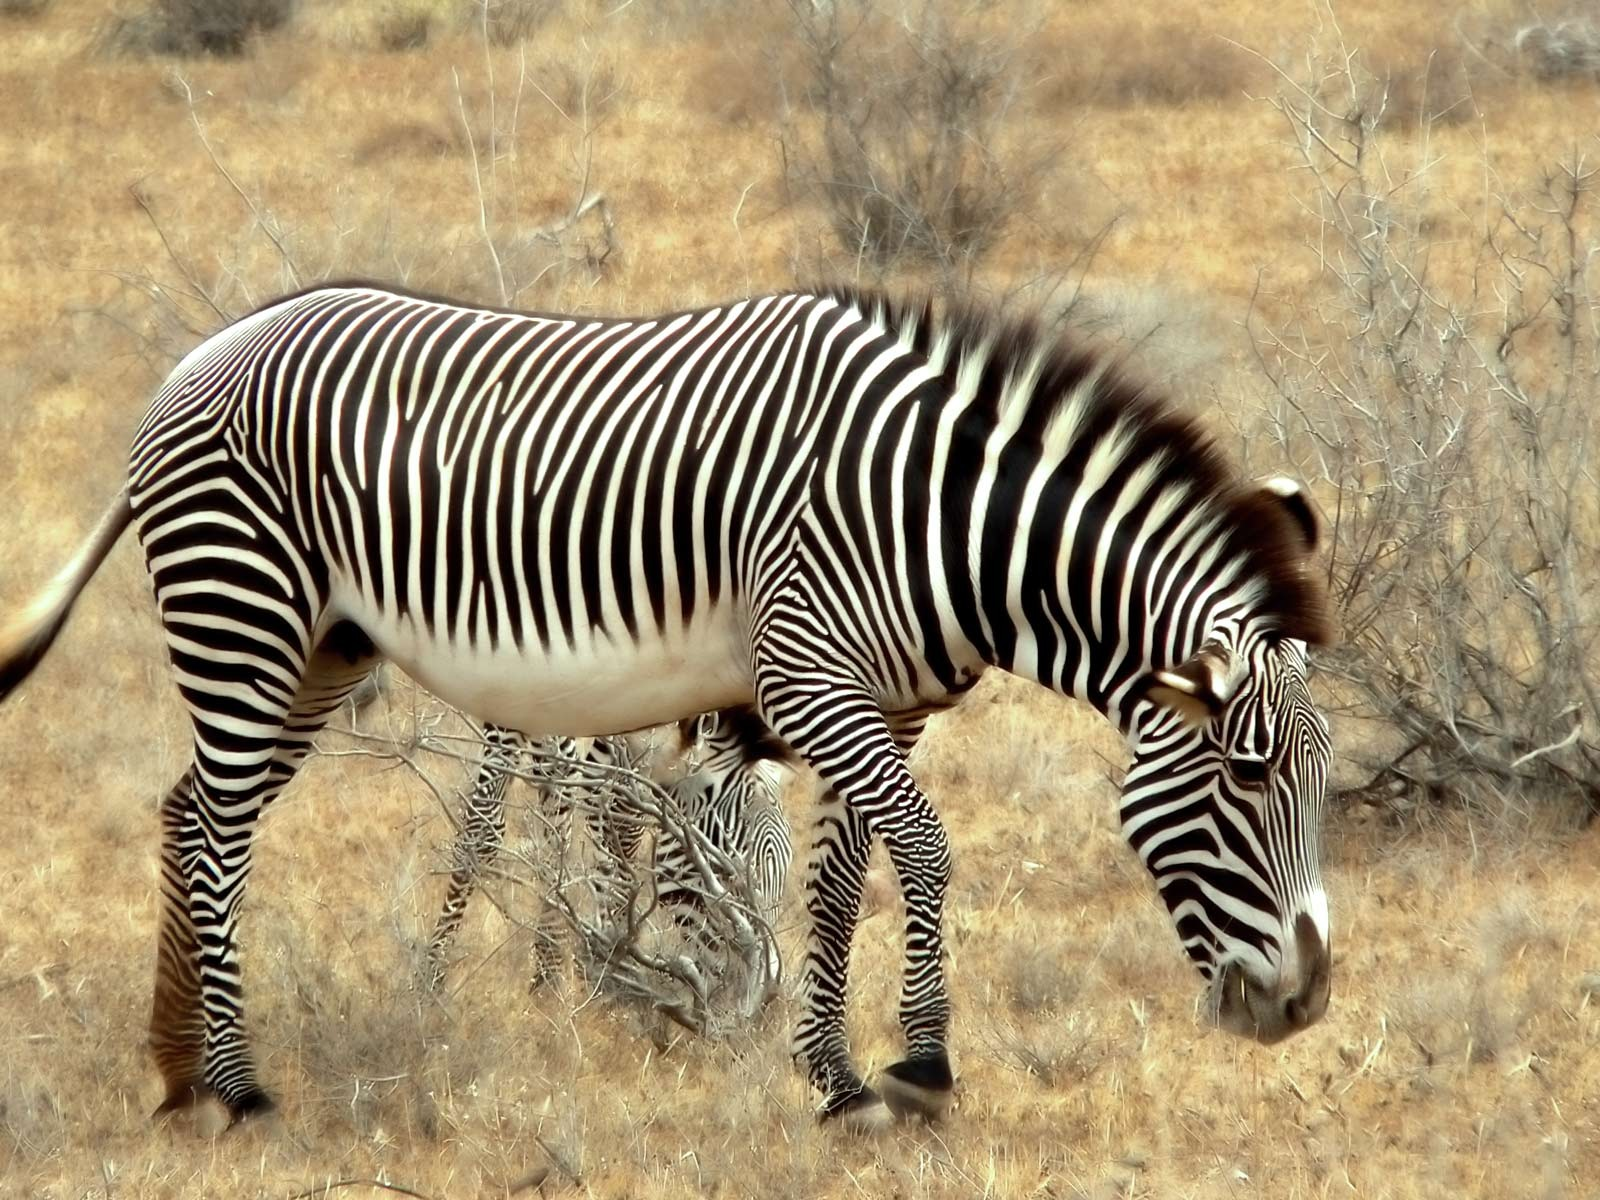
\includegraphics[width=0.3\textwidth]
{images/zebra}
\label{fig:zebra}}
\subfloat[]{
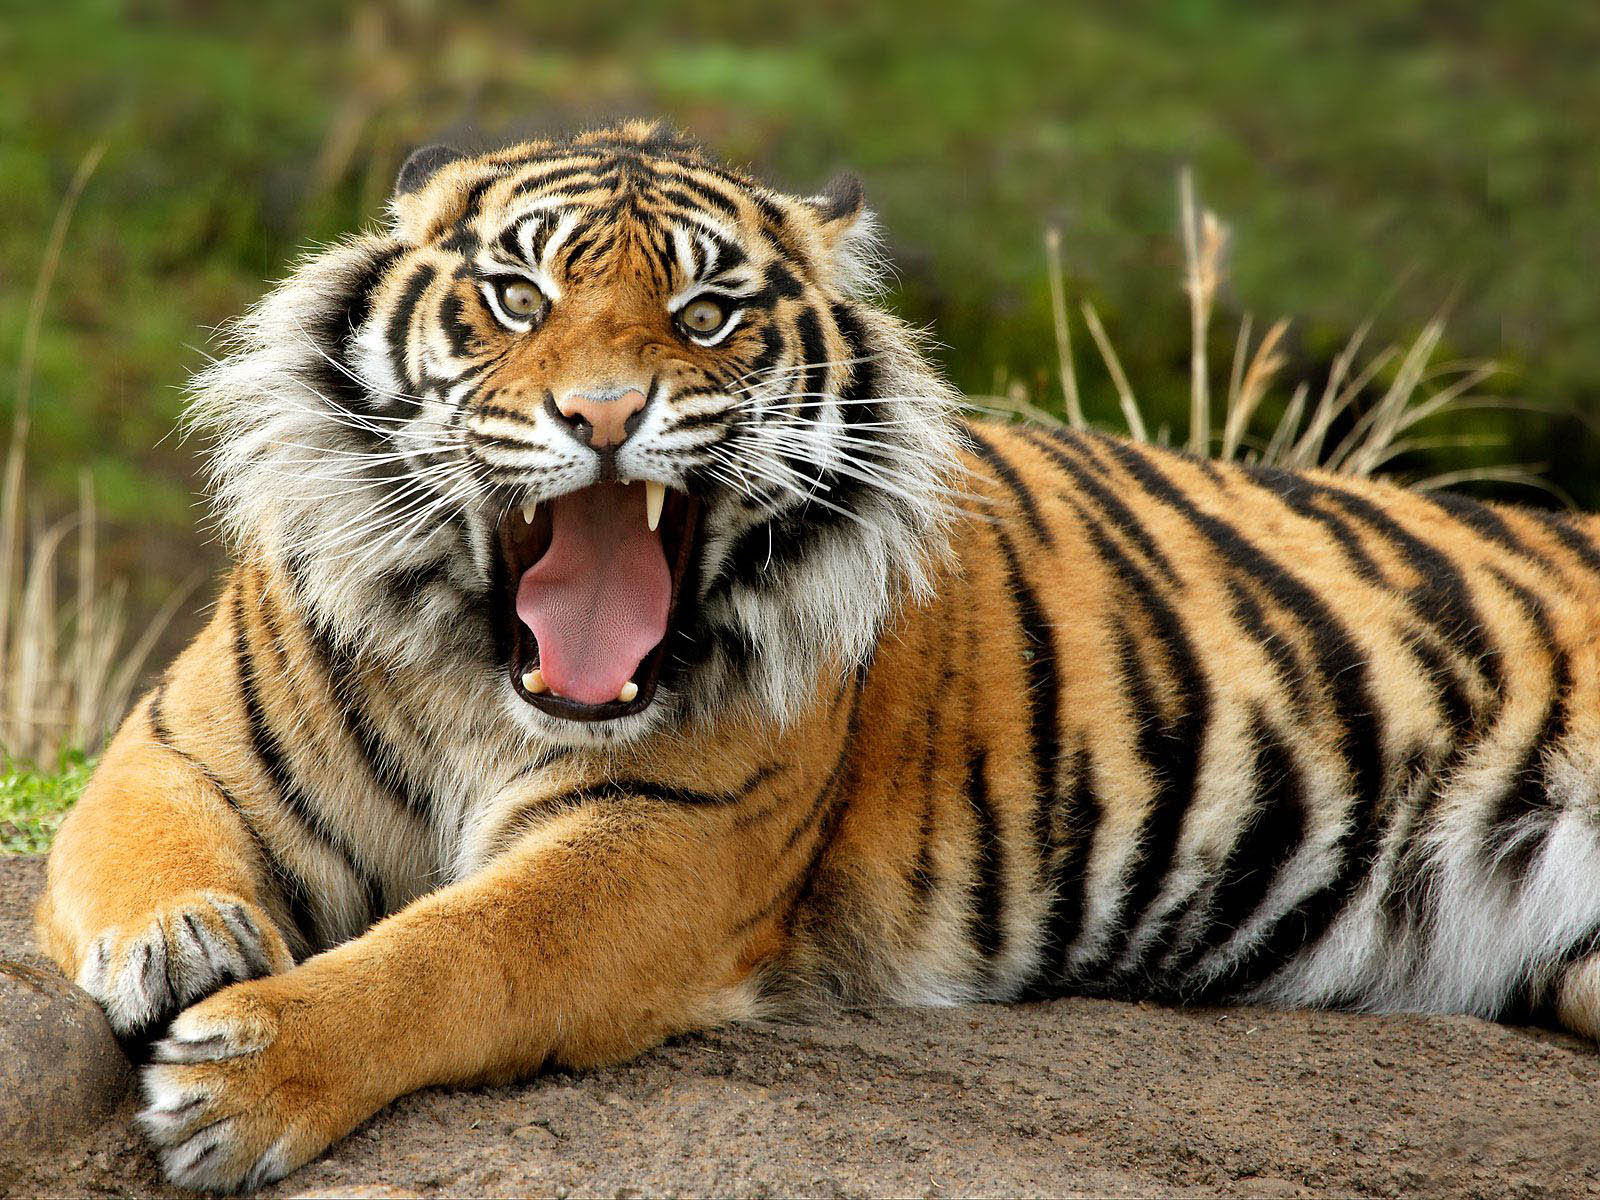
\includegraphics[width=0.3\textwidth]
{images/tiger}
\label{fig:tiger}}
\caption{Наслов на слика на македонски.}
\label{fig:animals}
\end{figure}

Екстра текст\index{текст}, екстра текст, екстра текст, екстра текст, екстра текст, екстра текст, екстра текст, екстра текст, екстра текст, екстра текст, екстра текст, екстра текст, екстра текст, екстра текст, екстра текст, екстра текст, екстра текст, екстра текст, екстра текст, екстра текст, екстра текст, екстра текст, екстра текст, екстра текст, екстра текст, екстра текст, екстра текст, екстра текст, екстра текст, екстра текст, екстра текст, екстра текст, екстра текст, екстра текст, екстра текст,

\begin{table}
\caption{Име на табелата}
\begin{tabular}{l*{4}{c}r}
Тим              & одиграни & победи & нерешени & порази & бодови \\
\hline
Манчестер Јун. & 6 & 4 & 0 & 2 & 12  \\
Селтик            & 6 & 3 & 0 & 3 &    9  \\
Бенфика           & 6 & 2 & 1 & 3 &    7  \\
ФК Вардар     & 6 & 2 & 1 & 3  &  7  \\
\end{tabular}
\end{table}

\section{Текст за следната слика}\label{something}
Бла бла бла текст за Слика~\ref{fig:bunchOfAnimals}), 
\begin{figure}[h!tb]
\centering
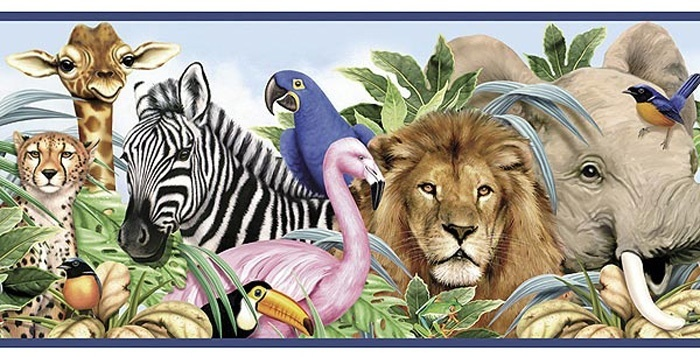
\includegraphics[width=0.8\textwidth]{images/animals}
\caption{This time, the text is in english.}
\label{fig:bunchOfAnimals}
\end{figure}

\chapter{Математика}
Ќе почнеме со следнава лема.
\begin{lemma} Сумата $\displaystyle\sum\limits_{i=0}^n i^3  = (\frac{n(n+1)}{2})^2$.
\end{lemma}
\begin{proof}
Доказот ќе го изведеме со помош на математичка индукција. За $n=1$ тврдењето важи:
\begin{align*}
\displaystyle\sum\limits_{i=0}^1 i^3  = (\frac{1(1+1)}{2})^2 = 1
\end{align*}
Да претпоставиме дека тврдењето важи за $n=k$ т.е. 
\begin{align}
\displaystyle\sum\limits_{i=0}^k i^3  = (\frac{k(k+1)}{2})^2 \label{eq:assumption}
\end{align}
Ако додадеме $(k+1)^3$ од обете страни на (\ref{eq:assumption})
\begin{align*}
\displaystyle\sum\limits_{i=0}^{k+1} i^3  = (\frac{k(k+1)}{2})^2 + (k+1)^3 &= (k+1)^2\frac{k^2 + 4k + 4}{4} = \frac{(k+1)^2(k+2)^2}{4}\\
& = (\frac{(k+1)(k+2)}{2})^2
\end{align*}
Значи тврдењето важи и за $n=k+1$. Според принципот на математичка индукција, тврдењето важи за секој $n$ природен број.
\end{proof}


\begin{corollary}фдсфсдфсдфќ ТТТ
\end{corollary}

На крајот ја имаме теоремата~\cite{big}
\begin{theorem}AAaтттт
\end{theorem}
\begin{proof}
\begin{align*}
\tg \alpha &= \ctg \beta \\
\arctg k &= \arcctg (2k)\\
\ldots & 
\end{align*}
Поради просторни ограничувања, остатокот од доказот е поместен во~\cite{small}. Со тоа теоремата е докажана.
\end{proof}

 
 \chapter{Малку подолг текст}
 
 Преземено од Википедија~\cite{website:WikipediaMacedonia}.
 
 \section{Македонија\index{Македонија}}
 
 Најпрво ќе почнеме со општи работи.
 
 \subsection{Општо}
 
 Македонија, или официјално Република Македонија — држава сместена на Балканскиот Полуостров. Земјата е една од наследничките држави на поранешната Југославија, од која прогласи независност во 1991 година. Република Македонија зафаќа околу 38\% од вкупната површина на регионот Македонија. Географски земјата граничи со Србија и Косово на север, Бугарија на исток, Грција на југ и Албанија на запад. Релјефот на државата е главно планински. Иако континентална држава, таа има повеќе од 50 езера и шеснаесет планини повисоки од 2.000 метри.

Македонија е суверена, самостојна, демократска и социјална држава. Главен град на државата е Скопје со население од 506.926 граѓани (проц. 2004). Други поголеми градови се: Битола, Куманово, Прилеп, Тетово, Велес, Штип, Охрид, Гостивар, Струмица, Кичево, Кавадарци и Кочани. Македони-ја има вкупно 25.713 километри квадратни во кои живеат околу 2.114.550 жители~\cite{website:ExampleWeb} (проц. 2009), од кои мнозинството се Македонци. Официјален јазик е Македонскиот јазик, додека официјална валута е Македонскиот денар.



\section{\emph{Пример за италик}}
Истото во италик

\emph{Македонија, или официјално Република Македонија — држава сместена на Балканскиот Полуостров. Земјата е една од наследничките држави на поранешната Југославија, од која прогласи независност во 1991 година. Република Македонија зафаќа околу 38\% од вкупната површина на регионот Македонија. Географски земјата граничи со Србија и Косово на север, Бугарија на исток, Грција на југ и Албанија на запад. Релјефот на држава-та е главно планински. Иако континентална држава, таа има повеќе од 50 езера и шеснаесет планини повисоки од 2.000 метри.\\
Македонија е суверена, самостојна, демократска и социјална држава. Главен град на државата е Скопје со население од 506.926 граѓани (проц. 2004). Други поголеми градови се: Битола, Куманово, Прилеп, Тетово, Велес, Штип, Охрид, Гостивар, Струмица, Кичево, Кавадарци и Кочани. Македо-нија има вкупно 25.713 километри квадратни во кои живеат околу 2.114.550 жители~\cite{website:ExampleWeb} (проц. 2009), од кои мнозинството се Македонци. Официјален јазик е Македонскиот јазик, додека официјална валута е Македонскиот денар.}

\chapter{Usage of other languages}

This is a very short demonstration of the \texttt{babel} package.

As you can see, it starts in English. However, the next paragraph will
be in Greek (actually, it will be in English, but written in Greek
script):



\selectlanguage{greek}
So this is in Greek script. I suppose you could use it for practicing
reading the  Greek alphabet.


\selectlanguage{english}
Now we are back in English again.

Today's date in English is \today, but in Greek it is 
\selectlanguage{greek}\today
\selectlanguage{english}, which looks different, but comes to the same
thing.

To get a better feel for what is possible, put in some tables,
and figures and \verb+\listoftables+ and \verb+\listoffigures+
commands, and make some language other than 
English the default.

\selectlanguage{french}
Maître Corbeau, sur un arbre perché,
Tenait en son bec un fromage.
Maître Renard, par l’odeur alléché,
Lui tint à peu près ce langage :
« Hé ! bonjour, Monsieur du Corbeau.
Que vous êtes joli ! que vous me semblez beau !
Sans mentir, si votre ramage
Se rapporte à votre plumage,
Vous êtes le Phénix des hôtes de ces bois. »
A ces mots le Corbeau ne se sent pas de joie ;
Et pour montrer sa belle voix,
Il ouvre un large bec, laisse tomber sa proie.
Le Renard s’en saisit, et dit : « Mon bon Monsieur,
Apprenez que tout flatteur
Vit aux dépens de celui qui l'écoute :
Cette leçon vaut bien un fromage, sans doute. »
Le Corbeau, honteux et confus,
Jura, mais un peu tard, qu’on ne l’y prendrait plus.

\selectlanguage{macedonian}

\section{Тест за останати кирилични карактери}

Test za kirilicni karakteri

Тест за кирилични карактери

\CYRG

\cyrzh

\'{\CYRG}

\CYRISHRT

\CYRJE

\CYRCH

\CYRDZHE

\CYRSH

\CYRNJE

\CYRLJE

\CYRDZE

\abstractname

\contentsname






\bibliographystyle{plain}
\bibliography{bibliography}
  
  \clearpage
  
    \prefacename
    
   \alsoname\\
    \seename\\
    
   
   \listoffigures
   \listoftables
 \printindex
    

\end{document}
